\subsection{EventMissedVerifier}

\subsubsection*{Code}

\inputgroovy[label=EventHandler.groovy]{../ChapterExercises/src/c9/EventHandler.groovy}

\inputgroovy[label=EventMissedVerifier.groovy]{../ChapterExercises/src/c9/EventMissedVerifier.groovy}

\subsubsection*{Results}

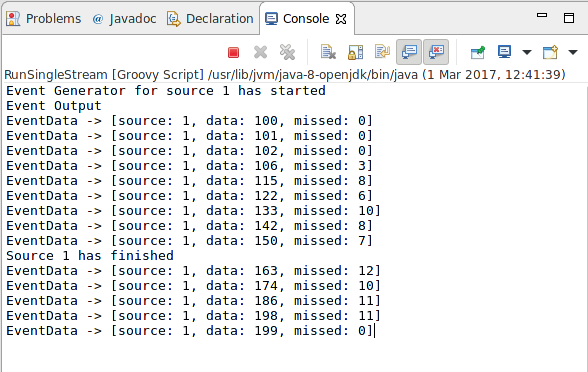
\includegraphics[width=\textwidth]{img/screenshots/9-1-1.png}

By changing the value of \textit{initialDataValue} to 0 we can see that the new class does throw an exception if the missed value is incorrect

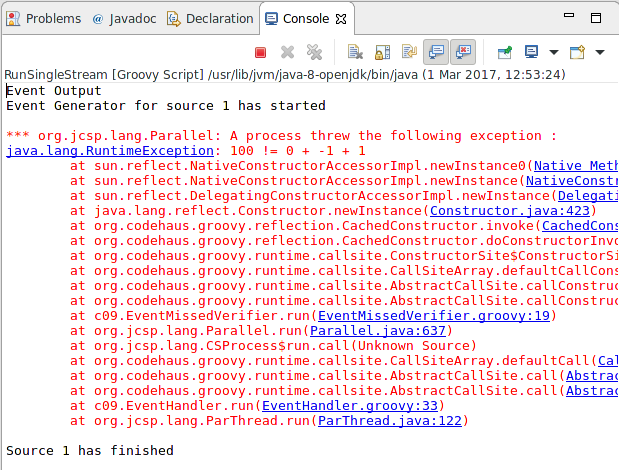
\includegraphics[width=\textwidth]{img/screenshots/9-1-2.png}
